\frontmatter
\chapter{前言}
Java系列教程分为两个部分:基础篇和提高篇,本书是第一部:基础篇。冒昧揣测,本书也可能
是国内第一本开源(open source)的Java8+教材,您可以在
\url{https://github.com/subaochen/java-tutorial}获得本书的所有源代码,
包括lyx源码、示例代码和图片等。

本书作为为数不多的涉及Java8+的教材,期望能够帮助读者在更高的平台上(本书放弃了
Java5之前的部分特性),在尽量短的时间内,掌握面向对象的基本思想、Java语言的
的基础语法和编程技能。

一般的,理工科院校讲授的第一门计算机程序设计语言是C语言,因此大家在学习(自学或者教学)
Java语言时已经具有了一定的C语言基础。而目前常见的Java语言教材或者辅导材料基本上
都是零基础开始讲授Java语言程序设计的,完全无视大家的C语言基础,导致教与学活动中
的很大浪费,也不利于突出Java教学活动的重点。因此,本书不是一本零基础的Java教程,
本书在很多章节将C语言和Java做了对比,引导读者从C语言转换到Java语言上来,笔者期望
读者在C语言的基础上能够实现Java语言的快速入门。

笔者斗胆计划在退休之前完成一个系列教程,也算是对教书生涯和以往工程实践经验的一个总结,
如图~\ref{fig:tutorial-plan}所示。

\begin{figure}[htbp]
    \centering
    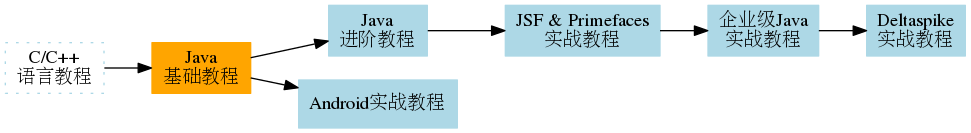
\includegraphics[width=\textwidth]{imgs/frontmatter/tutorials-plan}
    \caption{基于Java的系列教程计划}
    \label{fig:tutorial-plan}
\end{figure}

这有点类似于Java API,是一个公开的承诺,还望广大读者监督和鞭策!

\section*{本书的特点}
现有很多教材的示例代码往往过于随意,无论是类和变量的命名还是编程风格都欠缺规范,
而且可能只有一个片段,初学者很多时候不知道如何下手去验证作者的观点。可能是作者觉得
示例代码很短小,不值得精心雕琢吧。然而一本程序设计的教材,其示例代码却是精华所在,
读者可以借示例代码快速、准确的验证程序设计思路和作者的观点。因此,示例代码的规范化和
可随时验证就变得非常重要了。区别于这些传统教材的是,本书在编写示例代码时,全部经过笔者的
一手调试,并尽力保证类名、变量名等命名习惯以及编程风格(包括注释风格)接近工业标准,
以帮助读者从一开始就”先入为主“的了解正确的Java编程姿态。如果我们学习Java的目的是
对接工业化应用,笔者认为这样做可以事半功倍,也期待读者能够体会笔者的良苦用心。

本书注重从实战中学习Java的知识点,本书尽力做到每一个概念、每一个知识点都是可以验证的,
书中的每一个例子都是完整可运行的,都经过笔者的
亲自调试。本书的所有示例均可以从\url{https://github.com/subaochen/java-tutorial}
下载,笔者也会根据读者的反馈不断完善和调整示例程序。

本书通过思维导图的方式绘出了Java的各个知识点,并针对每个知识点设计了练习题,帮助
读者更好的了解这些知识点及其在实际中的应用方式。

本书尽力将知识点通过精确交叉索引(形如见xx节[在第yy页]的形式)的方式串接起来,以
方便读者了解知识点之间的关系。本书也特别强调了知识点出现的先后顺序,绝不使用后面
的知识解释前面的观点。

本书的例子均遵循google的编码规范(参考附录),希望读者在阅读本书示例代码的同时能够
直观的感受google编码规范并逐步养成遵守编码规范的好习惯。

\section*{本书读者对象}
\begin{itemize}
    \item 高校大二、大三的莘莘学子

        如果您已经学习过C语言,正打算深入学习一下Java,本书正是为您量身定做!尤其
        是大部分高校在大一安排学习C语言,本书可以作为大二学生的自学读物,或者后续
        开设Java程序设计语言课程时的教材,体现了知识体系的延续性。
    \item 没有程序设计语言的初学者
        
        如果您没有任何程序设计语言的基础,可能在阅读本书第二章时感觉有点过于简略,建议
        您适当补充一下关于程序设计语言的常识,比如数据类型、表达式、控制结构等。大部分
        程序设计语言在这些基础知识方面都是相通的,这也是本书假设读者在了解C语言的基础上,
        第二章内容非常简略的原因。
    \item 有一定程序设计语言的初学者
        
        虽然本书假设读者有一定的C语言基础,但是由于程序设计语言基础知识的共性很多,
        如果读者掌握了除C语言外的其他语言,比如Phthon等,阅读本书也没有任何困难。
    \item Java工程技术人员
        
        本书除了阐述Java的基本概念和编程方法外,也给出了常见的“最佳实践”供工程技术
        人员参考,也是本书学以致用原则的体现。
\end{itemize}

\section*{如何阅读本书}

本书不强调从一开始就掌握Java的每个技术细节,而是强调“先跑起来!”,即首先动手写出
一个可以运行的Java应用程序,并理解这个应用程序为什么能够跑起来,然后再逐步扩充到
细节问题。也就是说,在实践中体味和掌握技术细节,在实践中逐步形成良好的编程风格和
思维习惯。

笔者建议的阅读方式是:尽快、尽早的下载本书配套的示例代码,在阅读到例题的时候,
直接用Idea打开相应的项目即可查看和运行。同时,建议不要拘泥于笔者提供的示例代码,
读者完全可以也应该不断尝试修改并测试。编程能力就是在不断尝试中发展起来的。

本书也特别强调循序渐进的学习路线和知识的前后衔接以及连贯性。虽然Java语言经常存在
一个概念贯穿前后的情况,但是本书强调先掌握这个概念的部分特征,随着学习的深入,将
在后续章节逐步展开,并给出恰当的交叉索引将知识点逐步串联起来。

\iffalse
本教材特别强调学生主动参与的重要性。一般的,首先给出一个可以运行的简单示例,然后
通过不断提出问题的方式,让学生自己“探索”解决问题的方法,最终完成一个相当不错和有些
复杂的程序。通过这种方式将各个知识点串起来,弄清楚程序设计语言为什么这样设计和定义。
看起来一切都是学生自己完成的,这样学生的成就感很强,自学能力和自学的信心都会得到
很大程度的提高。
\fi

本书的章节标题如果是*开头的为较高要求内容,读者可以有选择的阅读,或者作为进阶的
阅读材料。


\section*{本书的体例}
\subsection*{印刷约定}
\begin{tabular}{|l|l|l|}
    \hline
    字体 & 意义 & 示例 \\
    \hline
    \textsl{AbCd123}斜体 & 文件名、路径名、域名等 & ls -l \textsl{filename}\\
    \hline
    \textbf{AbCd123}加粗 & 在终端输入的命令等 & subaochen\_desktop\% \textbf{su} \\
    \hline
    \texttt{等宽字体} & 示例代码、代码片段等 & \texttt{publc class MyClass...} \\
    \hline
\end{tabular}

\subsection*{图形标识}

本书使用了如下的图形标识帮助读者更好的区分和了解知识点所在:

\bgroup
\def\arraystretch{2.5}%
\begin{tabular}{ll}
\raisebox{-.4\height}{\includegraphics[width=8ex]{imgs/frontmatter/note.png}} & 需要注意的知识点。\\ 
\raisebox{-.4\height}{\includegraphics[width=8ex]{imgs/frontmatter/tip.png}} & 工程实践中常用的技巧。\\ 
\raisebox{-.4\height}{\includegraphics[width=8ex]{imgs/frontmatter/warning.png}} & 容易出错的地方,需要特别小心。\\ 
\end{tabular}
\egroup

\section*{如何使用本书的示例代码}
本书的每一个例题都附有完整可运行的示例代码,读者可以从\url{https://github.com/subaochen/java-tutorial}
下载本书的完整内容,其中在guide/code目录包含了示例代码。示例代码按照章节组织,
每个章节独立组织为一个Idea的项目,因此直接使用Idea打开所在章节的示例代码目录即可。

示例代码目录和章节的对应关系如下表所示:
\begin{center}
\begin{tabular}{c|c}
    \hline
    目录名 & 章节 \\
    \hline
    intro & 初识Java \\
    \hline
    verybasic & Java的基础语法 \\
    \hline
    oopbasic & 面向对象编程基础 \\
    \hline
    oopm & 面向对象工程思想 \\
    \hline
    essentials & Java的常用类 \\
    \hline
    exception & 异常处理 \\
    \hline
    io & Java的IO \\
    \hline
    enum & Enum \\
    \hline
    gui & 图形用户界面设计 \\
    \hline
    tests & 实验 \\
    \hline
\end{tabular}
\end{center}

\section*{联系笔者}
由于笔者的写作水平有限,本书难免存在不少的不妥之处,还请广大读者谅解并不吝指教。
您可以通过我的博客获得最新的消息:\url{http://dz.sdut.edu.cn/blog/subaochen},或者给
我发Email:subaochen@126.com。本书中的示例代码可以从\url{http://github.com/subaochen/
java-tutorial}下载,也欢迎读者不吝指教,在github提交PR,或者直接发邮件讨论亦可。
您可以在本书的不同章节看到如何获得源代码的相关提示。

\section*{本书是如何写成的}
本书全部使用开源(Open Source)软件完成:
\begin{itemize}
    \item Linux,本书所有稿件和源代码均在Linux下完成。
    \item git,本书的写作过程全程通过git进行版本控制,也借助于git在办公室、家和旅程中实现文档的同步,收益良多。
    \item Lyx(\url{http://www.lyx.org}),优秀的Latex前端可视化工具,最新版本
        (本书写作时是2.2)配合xetex、CTex可以很好的支持中文处理。
    \item graphviz,灵活而强大的代码绘图工具,本书部分流程图是使用graphviz绘制的。
    \item Shutter(\url{http://shutter-project.org}),Linux下面优秀的截图工具。
    \item ArgoUML(\url{http://argouml.tigris.org}),优秀的开源UML工具。
    \item umbrello(\url{https://umbrello.kde.org}),优秀的开源UML工具,本书部分UML图是使用umbrello绘制的。
    \item Dia,优秀的开源绘制工具,堪称Linux下面写作绘图的”瑞士军刀“,本书的大部分
        流程图、框图和UML图都是用Dia绘制的。
    \item Inkscape,优秀的开源矢量图绘制工具,本书的大部分矢量图是用Inkscape绘制的。
    \item vym(\url{http://www.insilmaril.de/vym/}),思维导图绘制工具,本书所有思维导图都是使用vym绘制的。
\end{itemize}

\section*{关于版权}
本书遵循Apache Licence,您可以在遵循Apache Licence和尊重原作者的的前提下,
在自己的博客、电子书等以电子文档的形式引用本书的内容,引用时请保留出处,
或者遵循常规的参考文献引用方式。

在本书正式出版前,笔者以及本书的其他贡献者一致要求,您不能将本书内容用于
正式出版物,包括但不限于本书的文字、图片和示例代码。

\section*{致谢}
\iffalse
写作如探险,一路坎坷,战战兢兢,如履薄冰。有的章节经过了屡次的推翻重来,
整本书的组织结构也经过了数次调整。在作为讲义内部使用的时候,学生们也给出了
很多中肯的建议和意见,笔者在授课过程中也不断的对本书的内容反思和整理。从构思
到成书,前后两年的时间,最终决定作为一本开源的Java系列教程。
\fi

感谢山东理工大学电气与电子学院对本书的资助,感谢各位同仁给予的帮助和指点,
感谢爱妻程玉华承担了大部分家务,让我有充足的时间专心写作;感谢实验室的小
伙伴们,尤其是胡安禄同学和徐千惠同学,帮助画出了部分示例图;感谢李松阳同学
在繁忙的工作之余认真校对,从标点符号到遣词造句都给出了很多具体的意见和建议。
如果您对本书的写作有所贡献,也会在这里一并感谢。如果有较大的贡献,本书正式
出版时将作为共同作者。期待更多的朋友加入进来!

特别的,要感谢我的女儿宿佳敏。写作本书时她正在读高中,笔者答应在这个寒假结束
时写完这本书送给她。我做到了,信守一个父亲的诺言。笔者坚信,这是最长情的陪伴和
对她学习的最好帮助。

在写作本书过程中,笔者查阅了大量Java教材和网络资料,所引用或依据的精彩论述和案例
尽量在文中标出,以便读者参照和比较,同时对原作者表示深深的敬意和感谢!

也感谢所有为开源软件作出贡献的人们!二十年前,当年懵懂的笔者决定彻底拥抱开源软件时,
为了安装一个Linux系统曾经不眠不休两天两夜;回头望,开源软件蓬勃发展二十年,
值得欣慰,值得弹冠相庆!没有Linux,没有Latex,没有Lyx,没有Dia,这本书也
不可能如此顺利的完稿。致敬,Open Source!

\hfill 宿宝臣

\hfill 2017年2月

\hfill 于山东理工大学1号实验楼
\mainmatter
